TJ-Monopix1 is a small electrode DMAPS with fast R/O capability, fabricated by TowerJazz foundry in 180 nm CMOS imaging process.
It is part, together with prototypes from other series such as TJ-MALTA, of the ongoing R$\&$D efforts aimed at developing DMAPS in commercial CMOS processes, that could cope with the requirements at accelerator experiments.
Both TJ-Monopix and TJ-MALTA series \cite{MALTA}, produced with the same technology by TowerJazz (the timeline of the foundry products is shown in figure \ref{fig:TJ180nm}), are small electrode demonstrators and principally differ in the readout design: while Monopix implements a column-drain R/O, an asynchronous R/O without any distribution of BCID has been used by TJ-Malta in order to reduce power consumption.

\begin{figure}[h!]
    \centering
    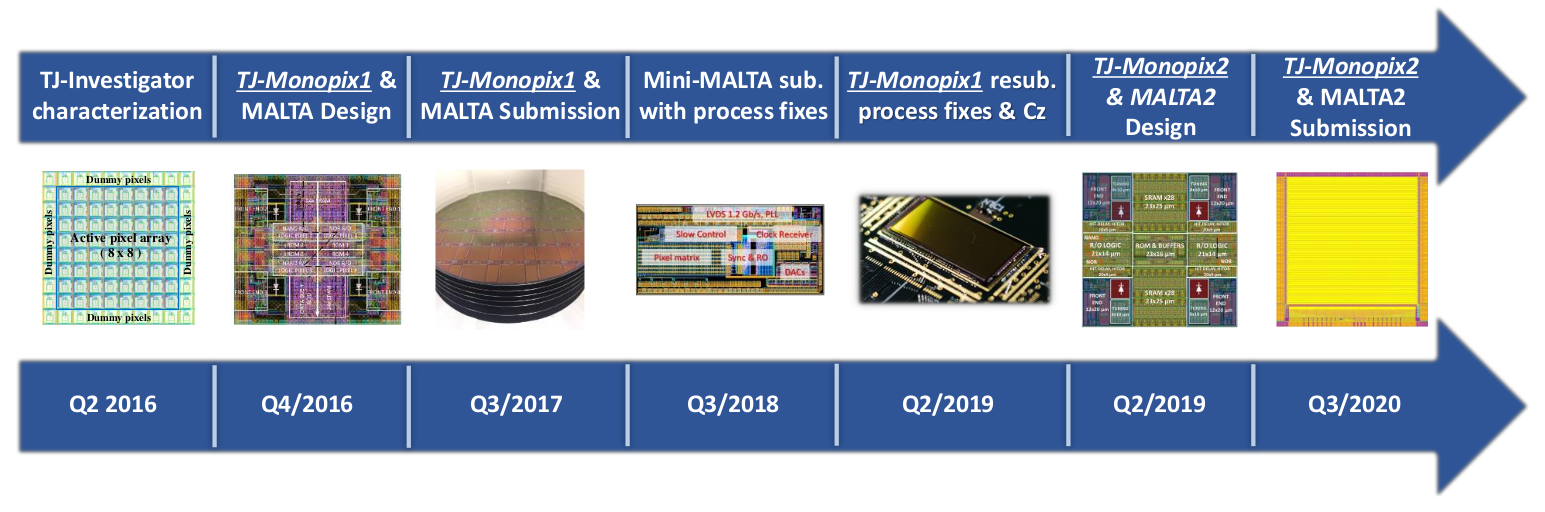
\includegraphics[width=.95\linewidth]{figures/Monopix1/TJ180nm.png}
    \caption{Timeline in TowerJazz productions in 180 nm CMOS imaging process}
    \label{fig:TJ180nm}
\end{figure} 

Another Monopix series, but in 150 nm CMOS technology, has been produced by LFoundry~\cite{LF-Monopix}.
The main differences between the LF-Monopix1 and the TJ-Monopix1 (summarized in table \ref{tab:LF-TJ-Monopix}), lay in the sensor rather than in the readout architecture, as both chips implements a fast column drain R/O with ToT capability \cite{LF-TJ-Monopix-short}\cite{LF-TJ-Monopix-long}.
Concerning the sensors, either are based on a p-type substrate, but with slightly different resistivities; in addition LFoundry pixels are larger, thicker and have a large fill factor (the very deep n-well covers $\sim$55$\%$ of the pixel area). The primary consequence is that LF-Monopix1 pixels have a higher capacity resulting in higher consumption and noise. As I discussed in section \ref{sec:small-large-fill-factor},  the fact that LF-Monopix has a large fill factor electrode is expected to improve its radiation hardness. Indeed, a comparison of the perfomance of the two chips showed that TJ-Monopix suffers a comparatively larger degradation of efficiency after irradiation, due to the low electric field in the pixel corner; on the other hand, a drawback of the large fill factor in LF-Monopix is a significant cross-talk.
\begin{table}
    \begin{center}
    \begin{tabular}{|c | c |c |}
    \hline
    & LF-Monopix1 & TJ-Monopix1\\
    \hline
    \hline
    Resistivity & $>$\SI{2}{k\Omega cm}& $>$\SI{1}{k\Omega cm}\\
    Pixel size & 50  $\times$ 250\si{\um\squared} & 36  $\times$ 40 \si{\um\squared} \\
    Depth & 100-750 \si{\um} & \SI{25}{\um} \\
    Capacity & $\sim$ \SI{400}{fF} & $\sim$ \SI{3}{fF}\\
    Preamplifier & charge & voltage \\
    Threshold trimming & on pixel (4-bit DAC) & global threshold\\
    ToT & 8 bits & 6 bits\\
    Consumption & $\sim$  300\si{mW/cm\squared}& $\sim$  120\si{mW/cm\squared} \\
    Threshold & 1500 $e^-$ & $\sim$ 270 $e^-$ \\
    ENC & 100 $e^-$ & $\sim$ 30 $e^-$\\
    \hline
    \end{tabular}
    \caption{Main characteristics of Monopix1 produced by TowerJazz and LFoundry \cite{LF-TJ-Monopix}}
    \label{tab:LF-TJ-Monopix}
    \end{center}
 \end{table}


\section{The sensor}
    TJ-Monopix1 adopts the modification described in section \ref{chap:a_modified_sensor} that allows to achieve a planar depletion region near the electrode applying a relatively small reverse bias voltage.
    This modification improves the efficiency of the detector, especially after irradiation, however a TCAD (Technology Computer Aided Design) simulation shows that a nonuniform electric field is still produced in the lateral regions compromising the efficiency at the pixel corner.
    On a sample of chip, which includes the one in Pisa, a second variation (fig. \ref{fig:Monopix1_section_scheme}) have been made to further enhance the transversal component of electric field: a portion of low dose implant has been removed, creating a step discontinuity in the deep p-well corner. 
    A side effect of the alteration in the low dose implant is the weaker separation between the deep p-well and the p-substrate, that cannot be biased separately anymore to prevent the punchthrough. 
    “extra deep p-well”.
        \begin{figure}[h!]
        \centering
        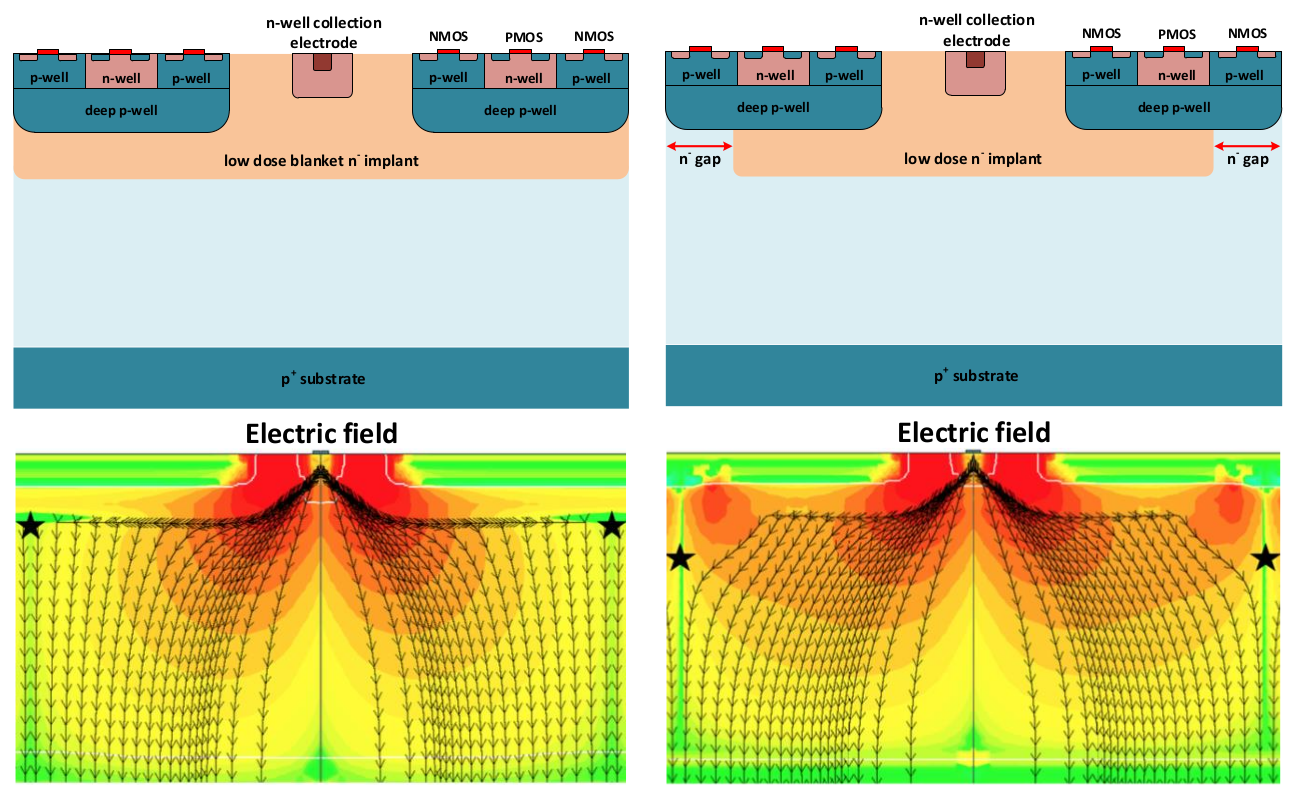
\includegraphics[width=.9\linewidth]{figures/Monopix1/Monopix1_section_scheme.png}
        \caption{(a) The cross-section of a monolithic pixel in the TJ-Monopix with modified process; additionally in (b) a gap in the low dose implant is created to improve the collection of charge due to a bigger lateral component of the electric field. this point in figure  is indicated by a star . transversal component of the electric field drops at the pixel corner}
        \label{fig:Monopix1_section_scheme}
    \end{figure}

    The collection electrode size is \SI{2}{\um} in diameter and its spacing from the electronics area is equal to \SI{3}{\um}, il deep p well è comune a tutti gli NMOS sul pixel
    Moreover, to investigate the charge collection properties, as the threshold, the noise and the efficiency, pixels within the matrix feature a difference in the doping structure of the deep p-well: rows from 0 to 111 are fully covered by deep p-well (FDPW), while rows from 112 till the last 223 have a portion of deep p-well removed (RDPW).

    The pixel electronics area of pixel belonging to the bottom
half of each column is fully covered by deep p-well (FDPW), while part of the deep p-well is removed (RDPW)
for pixels belonging to the top half of each column,
    The removing enhance the lateral electric field component then resulting in a higher efficiency, as we will see later.\\
    \red{The collection electrode size is
    2 \si{\mu m} in diameter and its spacing from the electronics area is equal to 3 \si{\mu m}; In order to reduce possible crosstalk, the digital and analog areas are
    physically separated}

\section{Front end}
    \begin{table}
        \begin{center}
        \begin{tabular}{| c |c |}
        \hline
        Parameter & Value\\
        \hline
        \hline
        Matrix size &  1 2\\
        Pixel size & 36 $\times$ 40 \si{\um\squared}\\
        Depth & \SI{25}{\um}\\
        Electrode size & \SI{2}{\um}\\
        BCID & \SI{40}{MHz} \\
        ToT-bit & 6 \\
        Power consumption & $\sim$ 120 \si{mW/cm\squared}\\    
        \hline
        \end{tabular}
        \caption{}
        \label{tab:LF-TJ-Monopix}
        \end{center}
    \end{table}
    The whole matrix contains 224 $\times$ 448 pixels, with size 36 $\times$ 40 \si{\mu^2} yielding a total active area approximately equal to 145 \si{mm^2} over a total area of 1 $\times$ 2 \si{cm^2}.
    In the chip periphery are placed all the required support blocks used for configuration and testing, while the matrix power pads are distributed at the sides.
    In particular, in the chip periphery, there are:  
    \begin{itemize}        
        \item some 7-bit Digital to Analog Converter (DAC), used to generate the analog bias voltage and current levels and to confiugure the FE
        \item a serializer is placed at the EoC to transferred datas immediately; no trigger memory is implemented in this prototypes, hence the R/O if full (continuous)
        \item four pixels which have analog output and which can be monitored with an oscilloscope, and therefore used for testing
    \end{itemize}
   
    \subsection{Four flavors}
        Four different flavors have been implemented in order to explore different variations of the data-bus readout circuitry and of the reset: each flavor corresponds to a different sector on the matrix(fig. \ref{fig:Monopix1_flavors}) and thus having a separate readout and data transmission. 
        \begin{figure}[h!]
            \centering
            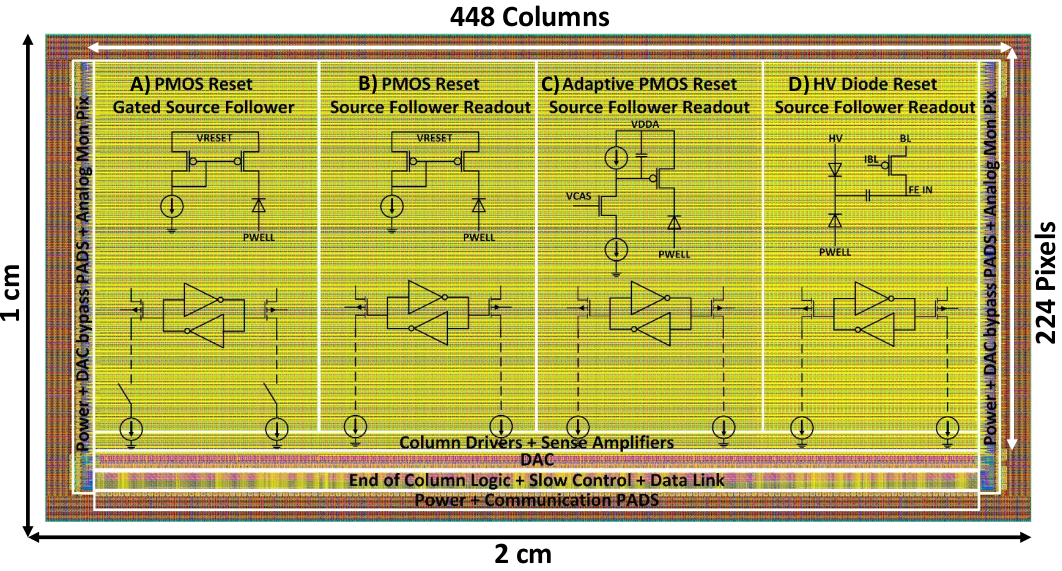
\includegraphics[width=.8\linewidth]{figures/Monopix1/Monopix1_flavors.png}
            \caption{}
            \label{fig:Monopix1_flavors}
        \end{figure}
        \red{Flavors B, C and D feature a source-follower column-bus readout derived from the LF-Monopix1 chip, that aims to reduce the crosstalk. However, it leads in a significant amount of static power being drawn at the EoC periphery. To elimnate static power consumption a modified gated source follower readout has been included in a flavor A, which is otherwise identical to flavor B. Flavor B, refereed to as the "PMOS reset", is the standard (reference ) variation and features a DC-couple PMOS input reset. Flavor C incorporates a novel leakage compensation circuit and flavor
        D, also called the "HV" flavor, explores the possibility of applying a high front-side bias voltage to the
        collection electrode which in this case is AC-coupled to the front-end input.}
        R resistenza di reset deve essere abbastanza grande in modo da far si che il ritorno allo zero è abbastanza lento (non devi "interferire" con la tot slope e non devi più corto del tempo del preamplificatore, sennò hai perdita di segnale).\\
        Baseline reset: all'input solitamente hai un PMOSS o un diodo;  
        \red{R reset; Voltage amplifier}
        The FE circuit \ref{fig:Monopix1_FE_circuit} is ALPIDE-like, so it is similar to the one described in \ref{chap:}; a quanto già detto voglio però aggiungere due parole: come viene implementato il mascheramento dei pixels e il reset.\\ 

    \subsection{ALPIDE-like front end}
        As I already mentioned, ALICE Pixel Detector (ALPIDE) is the current state-of-art and most of the following chips' FE are inspired by that, making it a standard in the FE design
        \begin{figure}[h!]
            \begin{subfigure}{.5\textwidth}
            \centering
            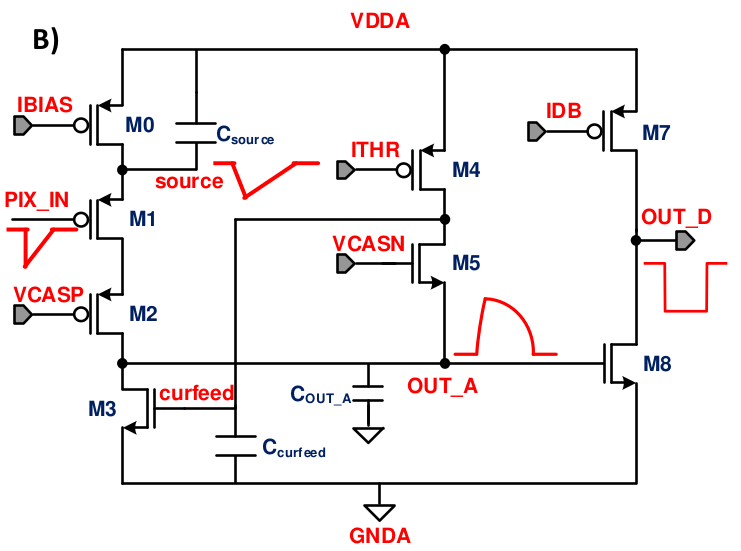
\includegraphics[width=.98\linewidth]{figures/Monopix1/ALPIDE_FE.png}
            \caption{ALPIDE-like}
            \label{fig:ALPIDE-like}
            \end{subfigure}
            \begin{subfigure}{.5\textwidth}
            \centering
            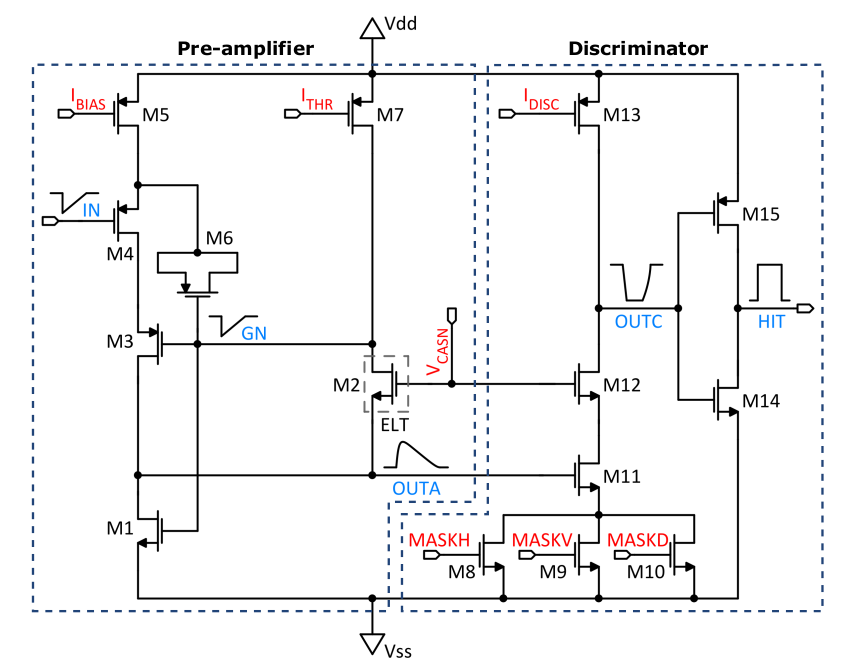
\includegraphics[width=.98\linewidth]{figures/Monopix1/Monopix1_FE_circuit.png}
            \caption{}
            \label{fig:Monopix1_FE_circuit}
            \end{subfigure}
        \end{figure}
        The idea of the amplification stage is to transfer the charge from a bigger capacity\cite{ALPIDE-FE}, $C_{source}$, to a smaller one, $C_{out}$: the input transistor M1 with current source IBIAS acts as a source follower and this forces the source of M1 to be equal to the gate input  $\Delta V_{PIX\_IN} = Q_{IN}/C_{IN}$.
        \begin{equation}
            Q_{source} = C_{source} \Delta V_{PIX\_IN}
        \end{equation}
        The current in M2 and the charge accumulates on $C_{out}$ is fixed by the one on $C_{source}$:
        \begin{equation}
            \Delta V_{OUT\_A} = \frac{Q_{source}}{C_{OUT\_A}} = \frac{C_{source}\Delta V_{PIX\_IN}}{C_{OUT\_A}}  = \frac{C_{Source}}{C_{OUT\_A}}\frac{Q_{IN}}{C_{IN}}
        \end{equation}
        A second branch (M4, M5) is used to generate a low frequency feedback, where VCASN and ITHR set the baseline value of the signal on $C_{OUT\_A}$ and the velocity to goes down to the baseline.\\
        \red{IL RUOLO DI CURVFEED NON L'HO CAPITO.}\\
        Finally IDB defines the charge threshold with which the signal $OUT\_A$ must be compared: depending on if the signal is higher than the threshold or not, the $OUT\_D$ is high or low respectively.
        I've already mentioned ALICE pixel dector talking about the new process modification, now the ALICE name comes up again talking about FE: this is because ALPIDE (ALice PIxel DEtector) is one of the first MAPS detector (TowerJazz 180 nm CMOS) installed \footnote{It was installed in the Inner Tracking System during the second long shut down of the LHC in 2019}, therefore it is the current state-of-art and most of the following chips' FE are inspired by that, making it a standard in the FE design.
            
        In order to reduce the hit rate and to avoid saturating the bandwidth, is uttermost important to include in the FE a way to mask noisy pixels, which typically are those with manufacturing defects.
        In the circuit in fig. \ref{fig:Monopix1_FE_circuit} transistors M8, M9 and M10 have the function of disabling registers with coordinates MASKH, MASKV and MASKD (respectivelly vertical, orizontal and diagonal) from readout: if all three transistors-signals are low, the pixel's discriminator is disabled. 
        Compared with a configurable masking register which would allow disableing pixels individually, to use a triple redundancy reduces the sensistivity to SEU\footnote{Single Event Upset, in sostanza è quando un bit ti cambia valore (da 0 a 1 o viceversa) perché una particella deposita carica nell'elettronica che fa da memoria registro/RAM/.... Questo tipo di elettronica ha bisogno di un sacco di carica prima che il bit si "flippi" (cambi valore), infatti tipicamente per avere un SEU non basta una MIP che attraversa esattemente quel pezzo di chip in cui è implementata la memoria, ma un adrone che faccia interazione nucleare producendo più carica di quanto farebbe una MIP. Questo metodo pur essendo più comodo richieda less amount of area ha però come drawback che il registro può essere soggetto a SEU problema non trascurabile in acceleratori come HL-LHC adronici} but also gives amount of intentionally masked ("ghost") pixels.
        This approach is suitable only for extremely small number N of pixel has to be masked: if two coordinate projection scheme had been implemented, the number of ghost pixels would have scale with $N^2$, if instead three coordinates are used, the N's exponential is lower than 2 (fig. \ref{fig:masking_scheme})
        \begin{figure}[h!]
            \centering
            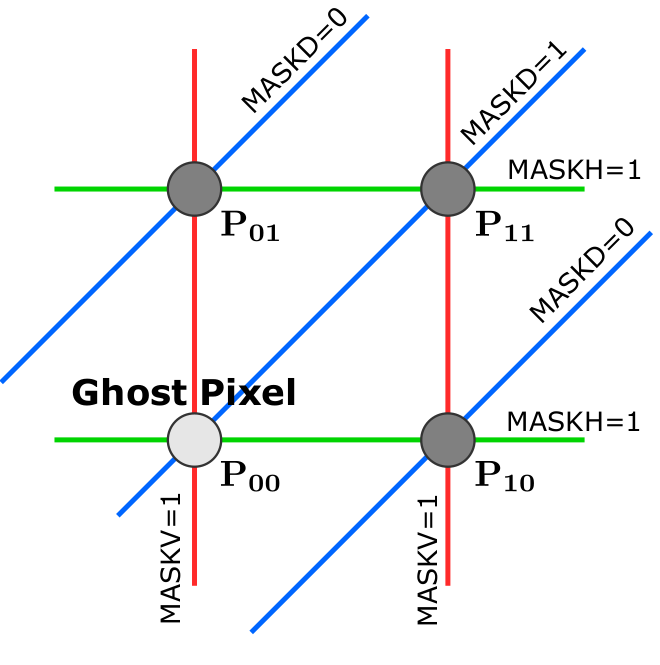
\includegraphics[width=.3\linewidth]{figures/Monopix1/masking_scheme.png}
            \caption{}
            \label{fig:masking_scheme}
        \end{figure}


    \subsection{Front end parameters}
        Descrivo un po' le misure fatte sul fe e sul significato dei vari parametri.\\
        it allows injecting pixels with a known charge in DAC units. 
        the front-end analog
        output of four special pixels at each side, placed next to the matrix, is buffered and can be monitored
        for characterization and debugging purposes.
        \begin{table}
            \begin{center}
            \begin{tabular}{|c | c |}
            \hline
            Parameter & Meaning\\
            \hline
            \hline
            IBIAS &\\
            IDB &\\
            ITHR & \\
            VCASN &\\
            VREF &\\
            IREF &\\
            \hline
            \end{tabular}
            \caption{}
            \label{tab:FE-parameters}
            \end{center}
        \end{table}
    
\section{Readout logic}
    TJ-Monopix1 has a triggerless, fast and with ToT capability R/O which is based on a column-drain architecture.      
    On the pixel are located two Random Access Memory (RAM) cells to store the 6-bit LE and 6-bit TE of the pulse, and a Read-Only Memory (ROM) containing the 9-bit pixel address. Excluded these memories, TJ-Monopix1 hasn't any other buffer: if a hit arrives while the pixel is already storing a previous one, the new data get lost.  
    After being read, the data packet is sent to the EoC periphery of the matrix, where a serializer transfers it off-chip to an FPGA (\ref{fig:R/O-system}). There a FIFO is used to temporarily stored the data, which is transmitted to a computer through an ethernet cable in a later time.  
    \begin{figure}
        \begin{subfigure}{\textwidth}
        \centering
        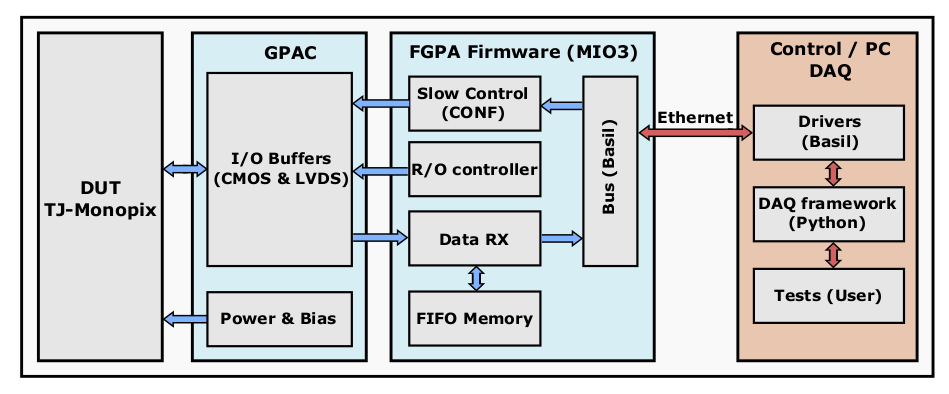
\includegraphics[clip,width=0.8\linewidth]{figures/Monopix1/schematic_boards.png}
        \end{subfigure}
        \bigskip
        \begin{subfigure}{\textwidth}
        \centering    
        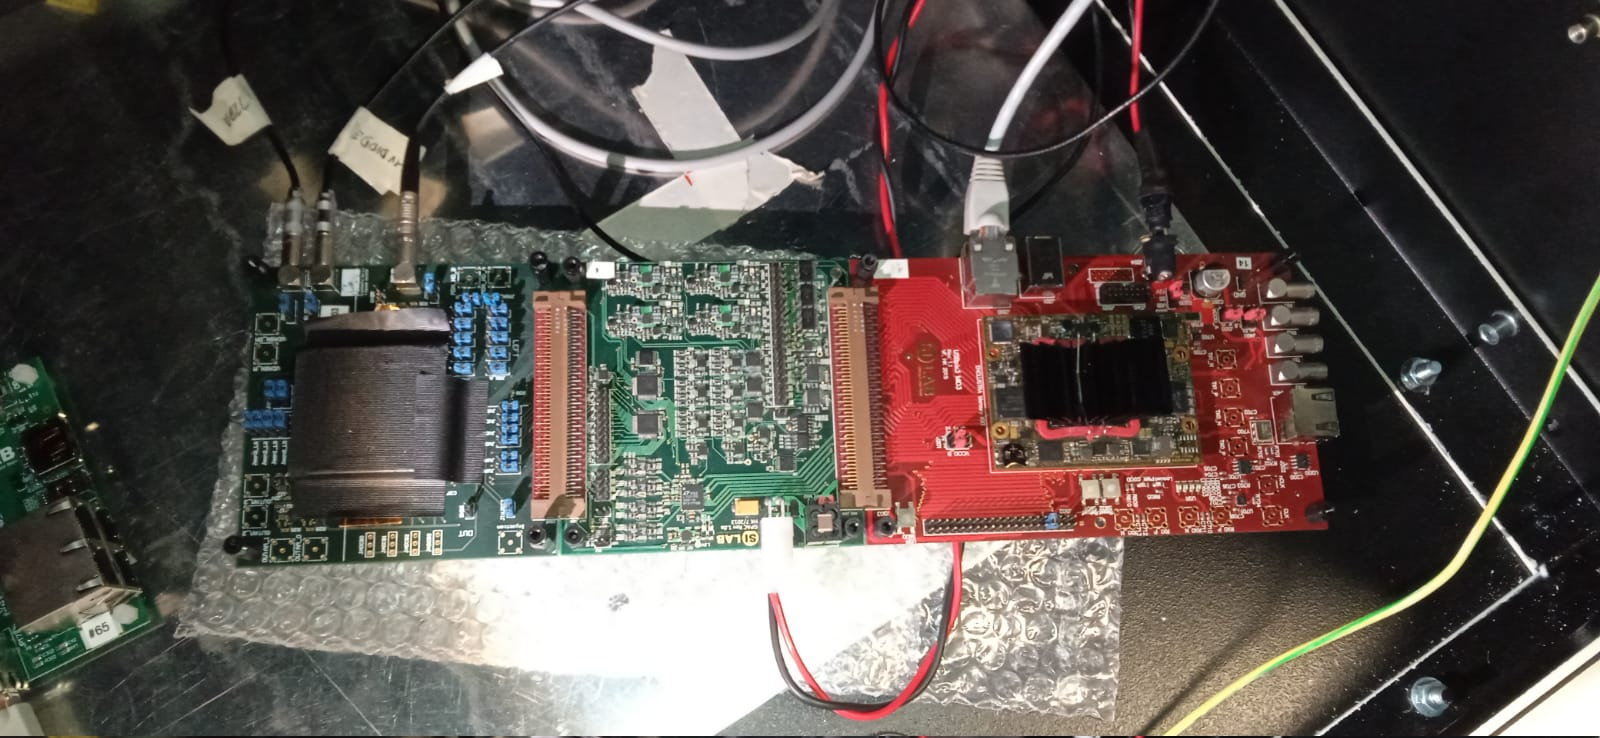
\includegraphics[clip,width=0.8\linewidth]{figures/Monopix1/monopix1_front.jpeg}
        \end{subfigure}
        \caption{Main caption}
        \label{fig:R/O-system}
    \end{figure}


    The access to the pixels' memory and the transmission of the data to the EoC, following a priority chain, is managed by control signals and is based on a Finite State Machine (FSM) composed by four state: no-operation (NOP), freeze (FRZ), read (RD) and data transfer (DTA). The readout sequence (\ref{fig:readout_schematics}) starts with the TE of a pulse: the pixel immediately tries to grab the column-bus turning up a hit flag signal called \textit{token}.   
    The token is used to control the priority chain and propagates across the column indicating what pixel that must be read. To start the readout and avoid that the arrival of new hits disrupt the priority logic, a \textit{freeze} signal is activated, and then a \textit{read} signal controls the readout and the access to memory.
    During the freeze, the state of the token for all pixels on the matrix remains settled: this does not forbid new hits on other pixels from being recorded, but forbids pixels hit from turning on the token until the freeze is ended. 
    The freeze stays on until the token covers the whole priority chain and gets the EoC: during that time new token cannot be turned on, and all hits arrived during a freeze will turn on their token at the end of the previous freeze.  
    Since the start of the token is used to assign a timestamp to the hit, the token time has a direct impact on the time resolution measurement; this could be a problem coping with high hits rate. 
    \begin{figure}[h!]
        \centering
        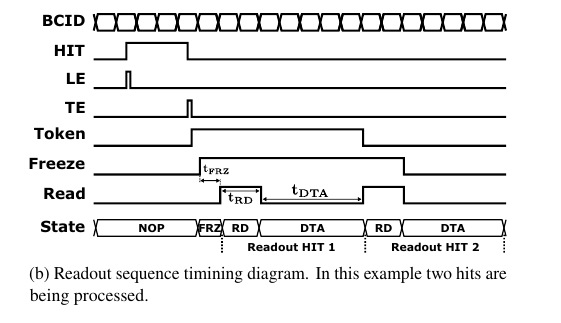
\includegraphics[width=.5\linewidth]{figures/Monopix1/readout_timing.png}
        \caption{Readout timing diagram: in this example two hits are being processed}
        \label{fig:readout_timing}
    \end{figure}

    The analog FE circuit and the pixel control logic are connected by an edge detector which is used to determine the LE and the TE of the hit pulse(fig. \ref{fig:pixel_logic}): when the TE is stored in the first latch the edge detector is disabled and, if the \textcolor{red}{FREEZE} signal is not set yet, the readout starts. 
    At this point the HIT flag is set in a second latch and a token signal is produced and depending on the value of \textcolor{Cerulean}{Token in} the pixel can be read or must wait until the \textcolor{Cerulean}{Token in} is off. In figure an OR is used to manage the token propagation, but since a native OR logic port cannot be implemented with CMOS logic, a sum of a NOR and of an inverter is actually used; this construct significantly increases the propagation delay (the timing dispersion along a column of 0.1-0.2 ns) of the token and to speed up the circuit optimized solution are often implemented.  
    When the pixel become the next to be read in the queue, and at the rising edge of the \textcolor{red}{READ} signal, the state of the pixel is stored in a D-latch and the pixel is allowed to use the data bus; the TE and the HIT flag latches are reset and a \textcolor{Cerulean}{READINT} signal that enable access of the RAM and ROM cells is produced.\\
    \begin{figure}[h!]
        \centering
        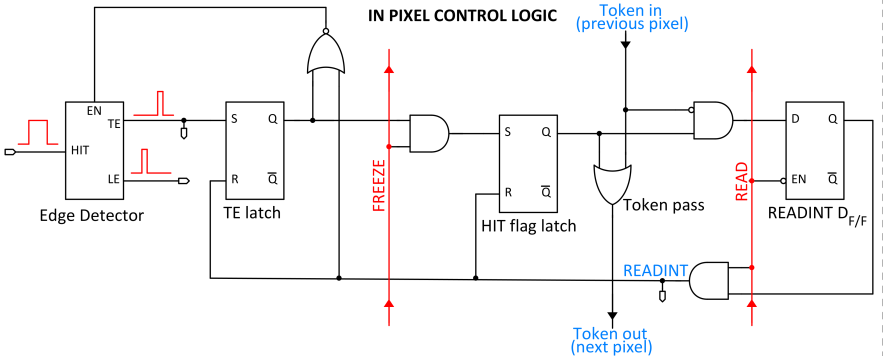
\includegraphics[width=.9\linewidth]{figures/Monopix1/Monopix1_readout_schematics.png}
        \caption{}
        \label{fig:pixel_logic}
    \end{figure}
    

    
    The final data must provide all the hits' information: the pixel address, the ToT and the timestamp. All those parts are assigned and appended at different time during the R/O chain:  
    \begin{itemize}
        \item\textbf{Pixel address:} while the double column address (6-bit) is appended by the EoC circuit, the row address (8-bits for each flavor) and the physical column in the doublet (1-bit) are assigned by the in-pixel logic      
        \item \textbf{ToT:} is obtained offline from the difference of 6-bits TE and 6-bits LE, stored by the edge detector in-pixel; since a 40 MHz BCID is distributed across the matrix, the ToT value is range 0-64 clock cycle which corresponds to 0-1.6 \si{\mu s}  
        \item \textbf{Timestamp:} The timestamp of the hit correspond to the time when the pixel set up the token; it is assigned by the FPGA, that uses the LE, TE and a 640 MHz clock to derive it. For all those hits which arrived while the matrix is frozen, the timestamp is no more correlated with the time of arrival of the particle         
    \end{itemize}
    When the bits are joined up together the complete hit data packet is 27-bit. 

    \subsection{Dead time measurement}
        The hit loss can be due to both analog and digital pile up: the first one occurs when a new hit arrives during the pre-amplifier response, the second instead occurs when a new hit arrives while the information of the previous hit has not yet been transferred to the periphery. 
        The digital pile-up contribution is the more relevant and the dead time is almost entirely determined by that; as only one hit at a time can be stored on the pixel's RAM, until the data have completed the path to get out, the pixel readout is paralyzed and the $\tau$ corresponds with the time needed to export the data-packets.
        Since the transmission of data from pixel to the EoC occurs via a \red{?}-bits data bus (this means that only one clock cycle is need to transfer the data to the end of column), the dead time bottleneck is given by the bandwidth of the serializer at the EoC: typically it operates at 40 MHz, and to transmit a data packet (27-bit) at least 675 \si{ns} are needed. 
        For what we have said so far, the R/O is completely sequential and therefore is expected a linear dependence of the reading time on the number of pixels to read:
        \begin{equation}
            \tau =\, 25\: \unit{ns}\, \times\, (\alpha\, N +\, \beta)
        \end{equation}
        where $\alpha$ and $\beta$ are parameters dependent on the readout chain. 
        In particular, looking at fig. \ref{fig:readout_timing}, $\alpha$ \red{is the time with $\alpha$ (CONF STOP FREEZE-CONF START READ), and $\beta$ ToT + CONF START FREEZE.}

        To measure and to test the linearity of the reading time with the number of pixels firing, I have used the injection mode available on the chip, that allows fixing not only the amplitude of the pulse (charge in DAC, as already seen in the previous section) but also the period and width.
        I have injected one hundred of pulses 
        Reducing each time the distance between two consecutive pulses, I have injected until the number of hits counted were less than the injected ones. 
        \red{Un esempio se leggo un singolo pixel: l'efficienza satura al 50\%}
        

        \red{Per definre meglio il $\tau$ faccio riferimento alla fig \ref{tempidilettura}: se una hit arriva su un pixel mentre ha il token alto allora la hit viene persa. Se una hit arriva su un pixel che non ha il token alto ma ha il freeze alto, allora non viene persa ma le viene assegnato un timestamp errato. PARLO ANCHE DELLA "RISOLUZIONE TEMPORALE?"} 
        \begin{figure}[h!]
                \centering
                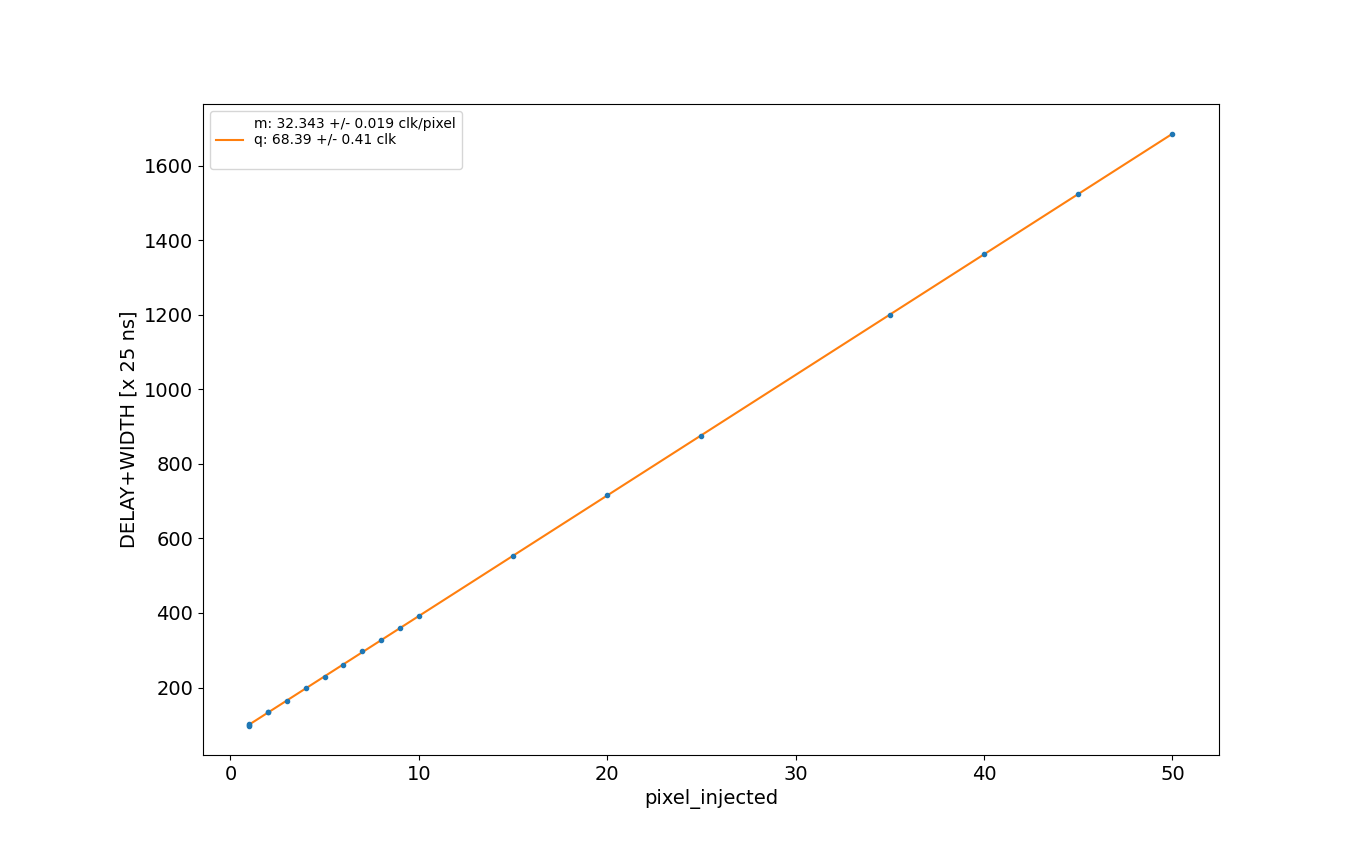
\includegraphics[width=.7\linewidth]{figures/Monopix1/dead_time.png}
                \caption{}
                \label{fig:dead_time}
            \end{figure}
        A tutte le hit di una iniezione che arrivano contemporaneamente viene assegnato lo stesso timestamp; quando le hit iniziano ad essere meno di quelle che mi aspetti.
        Mappa in funzione delle iniezioni di quali pixel hai letto.
        NON DIPENDE DALLA CARICA
    
